\documentclass{standalone}

%----------------------------------------------------------------------------------------------%
%                                 Packages and basic declarations
%----------------------------------------------------------------------------------------------%

\usepackage{amsmath}
\usepackage{mathrsfs}
\usepackage{pgf}
\usepackage{tikz}
\usepackage{verbatim}


\usetikzlibrary{arrows}



%----------------------------------------------------------------------------------------------%
%----------------------------------------------------------------------------------------------%
%                                            DOCUMENT STARTS
%----------------------------------------------------------------------------------------------%
%----------------------------------------------------------------------------------------------%

\begin{document}

%----------------------------------------------------------------------------------------------%
%                Single RVE with applied constant strain, only debonded
%----------------------------------------------------------------------------------------------%
 
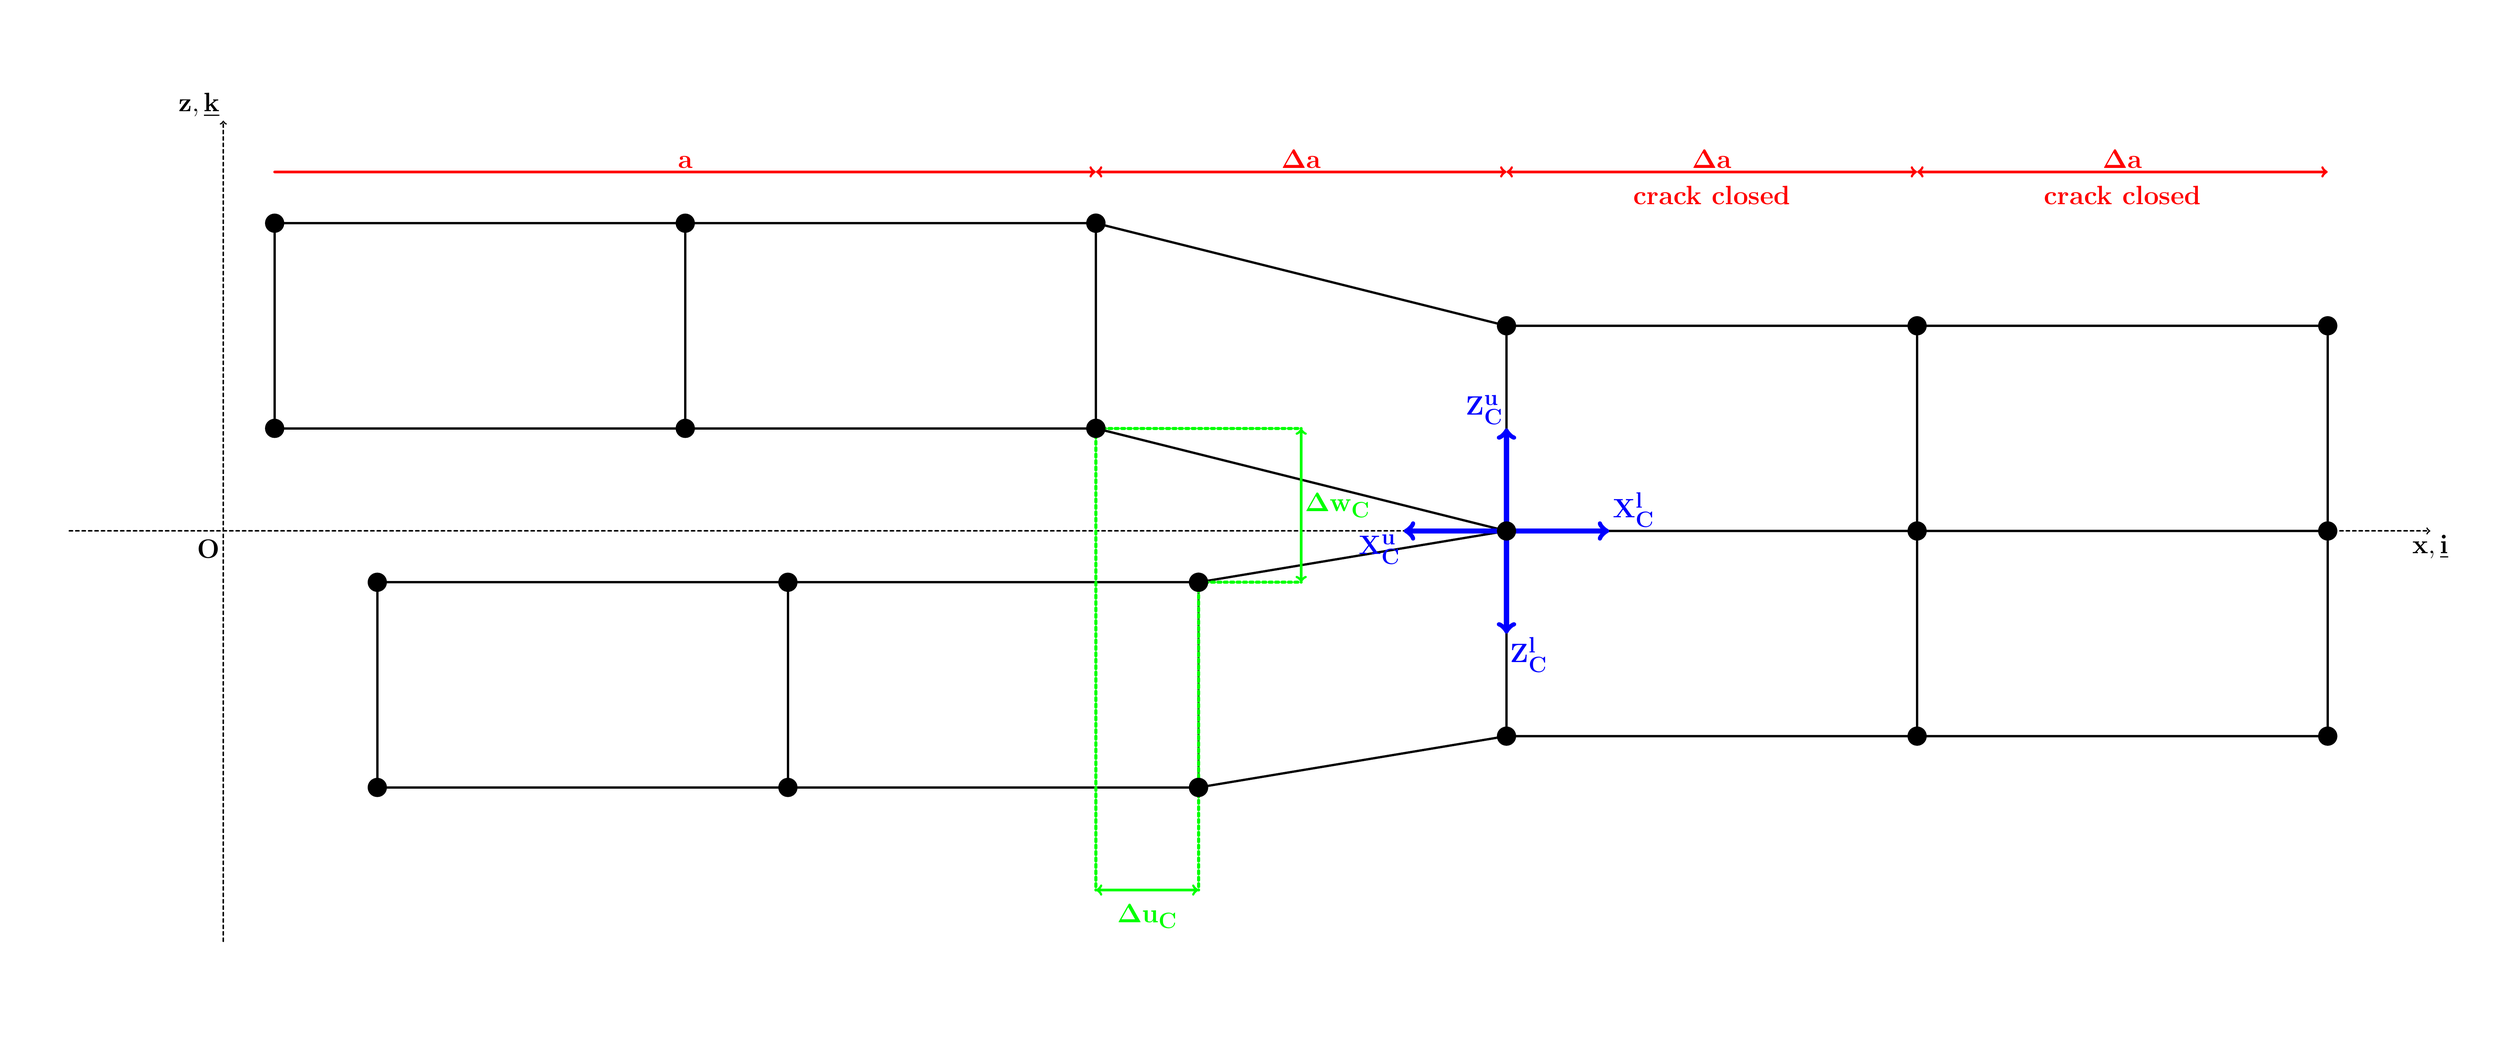
\begin{tikzpicture}[scale=4.5,cap=round,x=1.5cm,y=1.5cm]

%----------------------------------------------------------------------------------------------%
%                                                   CONSTANTS
%----------------------------------------------------------------------------------------------%

\def\pivalue{3.141592653589793238462643383279502884197169399375105820974944592307816406286}



\draw[->,dashed, line width = 0.5mm] (-7,0) -- (4.5,0);
\node[anchor=north] at (4.5,0) {\Huge $\mathbf{x,\underline{i}}$};
\draw[->,dashed, line width = 0.5mm] (-6.25,-2) -- (-6.25,2) ;
\node[anchor=south east] at (-6.25,2) {\Huge $\mathbf{z,\underline{k}}$};

\node[text=black,anchor=north east] at (-6.25,-0.025) {\Huge $\mathbf{O}$};

\draw[line width=0.75mm] (4,0) -- (4,1) -- (2,1) -- (0,1) -- (-2,1.5) -- (-2,0.5) -- (0,0) -- (2,0) -- (4,0);
\draw[line width=0.75mm] (4,0) -- (4,-1) -- (2,-1) -- (0,-1) -- (-1.5,-1.25) --  (-1.5,-0.25) -- (0,0);
\draw[line width=0.75mm] (4,1) -- (4,-1);
\draw[line width=0.75mm] (2,1) -- (2,-1); 
\draw[line width=0.75mm] (0,1) -- (0,-1);
\draw[line width=0.75mm] (-2,1.5) -- (-4,1.5) -- (-6,1.5) -- (-6,0.5) -- (-4,0.5) -- (-2,0.5);
\draw[line width=0.75mm] (-1.5,-1.25) -- (-3.5,-1.25) -- (-5.5,-1.25) -- (-5.5,-0.25) -- (-3.5,-0.25) -- (-1.5,-0.25);
\draw[line width=0.75mm] (-4,1.5) -- (-4,0.5);
\draw[line width=0.75mm] (-3.5,-1.25) -- (-3.5,-0.25);

\draw[<->,line width=0.9mm,draw=red] (0,1.75) -- (-2,1.75);
\node[anchor= south,text=red] at (-1,1.75) {\Huge $\mathbf{\Delta a}$};
\draw[->,line width=0.9mm,draw=red] (-6,1.75) -- (-2,1.75);
\node[anchor= south,text=red] at (-4,1.75) {\Huge $\mathbf{a}$};
\draw[<->,line width=0.9mm,draw=red] (0,1.75) -- (2,1.75);
\node[anchor= south,text=red] at (1,1.75) {\Huge $\mathbf{\Delta a}$};
\node[anchor= north,text=red] at (1,1.7) {\Huge \bf{crack closed}};
\draw[<->,line width=0.9mm,draw=red] (2,1.75) -- (4,1.75);
\node[anchor= south,text=red] at (3,1.75) {\Huge $\mathbf{\Delta a}$};
\node[anchor= north,text=red] at (3,1.7) {\Huge \bf{crack closed}};

\draw[dashed,line width=1mm,draw=green] (-1.5,-0.25) -- (-1.5,-1.75);
\draw[dashed,line width=1mm,draw=green] (-2,0.5) -- (-2,-1.75);
\draw[<->,line width=0.9mm,draw=green] (-2,-1.75) -- (-1.5,-1.75);
\node[anchor= north,text=green] at (-1.75,-1.8) {\Huge $\mathbf{\Delta u_{C}}$};


\draw[dashed,line width=1mm,draw=green] (-1.5,-0.25) -- (-1,-0.25);
\draw[dashed,line width=1mm,draw=green] (-2,0.5) -- (-1,0.5);
\draw[<->,line width=0.9mm,draw=green] (-1,-0.25) -- (-1,0.5);
\node[anchor= west,text=green] at (-1,-0.25+0.375) {\Huge $\mathbf{\Delta w_{C}}$};

\draw[->,line width=1.75mm,draw=blue] (0,0) -- (0,0.5);
\node[anchor=south east,text=blue] at (0,0.5) {\Huge $\mathbf{Z_{C}^{u}}$};
\draw[->,line width=1.75mm,draw=blue] (0,0) -- (0,-0.5);
\node[anchor=north west,text=blue] at (0,-0.5) {\Huge $\mathbf{Z_{C}^{l}}$};
\draw[->,line width=1.75mm,draw=blue] (0,0) -- (0.5,0);
\node[anchor= south west,text=blue] at (0.5,0) {\Huge $\mathbf{X_{C}^{l}}$};
\draw[->,line width=1.75mm,draw=blue] (0,0) -- (-0.5,0);
\node[anchor= north east,text=blue] at (-0.5,0) {\Huge $\mathbf{X_{C}^{u}}$};

\foreach \Point in {(4,0) , (4,1) , (2,1) , (0,1) , (-2,1.5) , (-2,0.5) , (0,0) , (2,0),(4,-1) , (2,-1) , (0,-1) , (-1.5,-1.25) ,  (-1.5,-0.25),(-2,1.5) , (-4,1.5) , (-6,1.5) , (-6,0.5) , (-4,0.5) , (-2,0.5),(-1.5,-1.25) , (-3.5,-1.25) , (-5.5,-1.25) , (-5.5,-0.25) , (-3.5,-0.25) , (-1.5,-0.25)}{
    \fill \Point  circle[radius=2pt];
}

\node[anchor= south,text=red] at (-1,2.5) {};
\node[anchor= north,text=red] at (-1.75,-2.5) {};
\node[anchor= east,text=red] at (-7.25,0) {};
\node[anchor= west,text=red] at (4.75,0) {};


\end{tikzpicture}

\end{document}